\documentclass[a4paper,UKenglish]{dagrep-v2018}

\usepackage[utf8]{inputenc}
\usepackage{microtype}
\usepackage{graphicx}

\bibliographystyle{plain}

\iffalse
\usepackage{draftwatermark} % option '[nostamp]' to ignore watermark
\SetWatermarkFontSize{5cm}
\SetWatermarkScale{0.5}
\SetWatermarkLightness{0.8}
\SetWatermarkColor[rgb]{0.95,0.4,0.1}
\SetWatermarkText{\shortstack[l]{\vspace*{3cm}\ \textsf{DRAFT 2020-01-08}}}
\fi

\subject{Report from Dagstuhl Seminar 19442}
\title{Programming Languages for Distributed Systems and Distributed Data Management}
\titlerunning{19442 -- Programming Languages for Distributed Systems and Distributed Data Management}

\author[1]{Carla Ferreira}
\author[2]{Philipp Haller}
\author[3]{Volker Markl}
\author[4]{Guido Salvaneschi}
\author[5]{Cristina Videira Lopes}
\authorrunning{Ferreira, Haller, Markl, Salvaneschi, and Videira Lopes}
\affil[1]{Universidade NOVA de Lisboa, PT, \texttt{carla.ferreira@fct.unl.pt}}
\affil[2]{KTH Royal Institute of Technology - Stockholm, SE, \texttt{phaller@kth.se}}
\affil[3]{TU Berlin, DE, \texttt{volker.markl@tu-berlin.de}}
\affil[4]{TU Darmstadt, DE, \texttt{salvaneschi@st.informatik.tu-darmstadt.de}}
\affil[5]{University of California - Irvine, US, \texttt{lopes@uci.edu}}

\seminarnumber{19442}
\semdata{October 27--31, 2019 -- \href{http://www.dagstuhl.de/19442}{http://www.dagstuhl.de/19442}}

\volumeinfo%(easychair interface)
  {Carla Ferreira, Philipp Haller, Volker Markl, Guido Salvaneschi, and Cristina Videira Lopes}%editor names
  {5}%number of editors
  {Programming Languages for Distributed Systems and Distributed Data Management}%seminar title
  {9}%volume
  {10}%issue
  {1}%starting page number
\DOI{10.4230/DagRep.9.10.1}%(DagRep.<volume no>.<issue no>.<firstpage>)

\begin{document}

\maketitle

\begin{abstract}
Programming language advances have played an 
important role in various areas of distributed systems research, including 
consistency, communication, and fault tolerance, enabling automated reasoning
and performance optimization.
% for distributed systems have been flourishing in the past, 
% providing ideas for the development of complex systems that 
% have been deeply influential.
However, over the last few years, researchers focusing on this area 
have been scattered across different communities such as
language design and implementation, (distributed) databases,
Big Data processing and IoT/edge computing -- resulting in limited interaction.
The goal of this seminar is to build a community of researchers interested in
programming language techniques for distributed systems and distributed data management, 
share current research results and set up a common research agenda. 
This report documents the program and the outcomes of Dagstuhl Seminar 19442 ``Programming Languages for Distributed Systems and Distributed Data Management.''
\end{abstract}

\section{Summary}

Developing distributed systems is a well-known, decades-old problem in computer science. Despite significant research effort dedicated to this area, programming distributed systems remains challenging. The issues of consistency, concurrency, fault tolerance, as well as (asynchronous) remote communication among heterogeneous platforms naturally show up in this class of systems, creating a demand for proper language abstractions that enable developers to tackle such challenges.

Over the last years, language abstractions have been a key for achieving the properties above in many industrially successful distributed systems. For example, MapReduce takes advantage of purity to parallelize task processing; complex event processing adopts declarative programming to express sophisticated event correlations; and Spark leverages functional programming for efficient fault recovery via lineage. In parallel, there have been notable advances in research on programming languages for distributed systems, such as conflict-free replicated data types, distributed information-flow security, language support for safe distribution of computations, as well as programming frameworks for mixed IoT/cloud development.

However, the researchers that have been carrying out these efforts are scattered across different communities which include programming language design, type systems and theory, database systems and database theory, distributed systems, systems programming, data-centric programming, and web application development. This Dagstuhl Seminar brought together researchers from these different communities.

The seminar focused on answering the following major questions: %in addition to those raised by participants:

\begin{itemize}

\item Which abstractions are required in emergent fields of distributed systems, such as mixed cloud/edge computing and IoT?

\item How can language abstractions be designed in a way that they provide a high-level interface to programmers and still allow fine-grained tuning of low-level properties when needed, possibly in a gradual way?

\item Which compilation pipeline (e.g., which intermediate representation) is needed to address the (e.g., optimization) issues of distributed systems?

\item Which research issues must be solved to provide tools (e.g., debuggers, profilers) that are needed to support languages that target distributed systems?

\item Which security and privacy issues come up in the context of programming languages for distributed systems and how can they be addressed?

\item What benchmarks can be defined to compare language implementations for distributed systems?
\end{itemize}

The seminar accomplished the goal of bringing together the research communities of databases, distributed systems, and programming languages. The list of participants includes  24 academic and industrial researchers from Austria, Belgium, France, Germany, Portugal, Sweden, Switzerland, UK, and USA, with complementary expertise and research interests. 
The group had a balanced number of senior researchers and junior researchers, as well as a strong industrial representation.

The scientific program comprised 28 sessions. The sessions devoted to individual presentations included 16 short talks with a maximum duration of 15 minutes and 6 long contributed talks with a maximum duration of 35 minutes.
In addition, the seminar included 2 plenary sessions and 4 group sessions. 
The first two days of the seminar were dedicated to research talks, but it was ensured that each talk had  
allocated time for discussions and exchange of ideas. In the two following mornings there were 3 plenary sessions and 2 parallel group sessions.
The topics for these sessions were proposed and selected after a lively discussion between participants, 
where the most popular sessions were promoted to plenary and the remaining occurred in two parallel sessions.
The scientific sessions discussed and collected open questions on the topics of: programming models and abstractions; security and privacy; 
static guarantees, type systems, verification; distributed computing for the edge; time, synchrony, and consistency; and persistency and serialization. There was also a social topic discussing further actions to bring the three communities together. Even though there are overlapping research interests, there is a difference of values between communities that needs to be acknowledged and tackled.
Participants agreed on the goal of organizing follow-up events to further strengthen the connection
among the database, the distributed systems and the programming languages communities. In particular, the importance of extending future events to Ph.D. students, for instance with an integrated Summer School, has been discussed.
%As a result of the seminar participants from these different communities starting discussing new collaborations and planning future events.

%\begin{itemize}
%\item Programming models (plenary):  What should be the abstractions exposed to application programmers?
%What is a better approach, multitier programming or transparently deriving distributed program from a sequential one?
%How to organizes the layers / stack in distributed systems? 
%Layers / stack in distributed systems: how to organize the system, composition
%\item  Security and privacy (plenary): When is security not orthogonal? Common vocabulary?  Privacy and trust, provenance
%\item Social topic (plenary): DS community, DB community and PL community? How can the two communities benefit from each other? How to bridge different communities? Follow up event?
%\item Static guarantees, type systems, verification (group): 
%\item Distributed computing for the edge (group): 
%\item Time and synchrony (group):  Integrating time into PL. Consistency
%\item Persistence (group): Most PL are not designed for persistence, typing 
%Materialization, view updates
%Data and control, database management 
%\end{itemize}


\tableofcontents

% Overview of Talks %%%%%%%%%%%%%%%%%%%%%%%%%%%%%%%%%%%%%%%%%%%%%%%%%%%%%%%%%%%%%%%%%%%%%%%%%%%%%%%%

\section{Overview of Talks}

%%%%%%%%%%%%%%%%%%%%%%%
\abstracttitle{Aggregation $\neq$ Replication}
\abstractauthor[Carlos Baquero]{Carlos Baquero (Universidade do Minho -- Braga, PT, cbm@di.uminho.pt)}

\license

Both distributed aggregation and replication for high availability are techniques that can help tackle geo-replication, offline operation and edge/fog computing. Distributed aggregation often shares many properties in common with CRDT style convergent replication, but they are not the same concept. 
The main difference is that in replication there is an abstraction of a single replicated state that can be updated in the multiple locations where a replica is present. This state is not owned by any given replica, but any replica can evolve it by applying operations that transform the shared state. This notion applies both in strong consistency and high availability settings. The difference being that in highly available replication the replicas are allowed to diverge and later reconcile. Another factor is that operations that lead to state changes are often the result of the activity an external user that interacts with the system, e.g. adjusting the target room temperature up by 2 degrees. As such, different users, can do conflicting actions, either concurrently or in sequence (most of us did in their childhood on/off light switching fights with other kids and adults).

Distributed data aggregation refers to several data aggregation techniques that are common in sensor network settings and datacenter infrastructure monitoring. In contrast to replication, each node/location has access to its own local data, e.g. CPU utilisation or a local measurement of humidity levels, and typically this data can evolve continuously. Also, the data to be aggregated is often not directly controlled by users, it usually results from an external physical process or the result of complex system evolutions. Thus, each sensing node usually has exclusive access to a local input value that evolves in time. The aggregation process is then tasked with collecting and transforming this information, e.g. calculating the average or the maximum value, and making it available at a specified location (sink) or disseminating it back to the nodes (by broadcasting the aggregate result). In aggregation the source of truth for each individual measurement is in the actual node that provided it.

Sometimes the two concepts have in common the notion of data merging. In state-based CRDTs operations are reflected in a semi-lattice state that can be combined with others with a join function. In data aggregation there is also often a notion of joining data together, but there is an additional aspect of data reduction and summarisation that is usually not present in CRDT designs. To add to the confusion, it’s is possible to combine the two concepts in a single system, as we did in the design of Scalable Eventually Consistent Counters, that combines a hierarchical CRDT design with a global aggregation and reporting facet.
However, ignoring corner cases, the difference can be quite clear and recognising it can help in selecting the right tools. A final take-away example is to consider the control of room temperature: The plus/minus control that sets the set point temperature can be captured by a CRDT; The combining of different temperature sensors across the room to obtain the average temperature is distributed aggregation.

%%%%%%%%%%%%%%%%%%%%%%%
\abstracttitle{Stateful serverless programming}
\abstractauthor[Sebastian Burckhardt]{Sebastian Burckhardt (Microsoft Research Lab -- Redmond, US, sburckha@microsoft.com)}

\license

Serverless programming models, such as AWS Lambdas or Azure Functions, simplify the development of elastic cloud services by automating low-level aspects of deployment, VM management, and monitoring. However, building a stateful application from stateless functions still poses some challenges for developers, such as handling partial execution failures, or enforcing proper synchronization of conflicting operations. In Azure Durable Functions we offer several features to aid developers in that regard: orchestrations provide reliable workflows, entities provide reliable application objects, and critical sections provide reliable multi-object synchronization. The resulting programming model combines aspects of both the actor model and shared memory, but can execute reliably in a distributed serverless context, and is guaranteed to not deadlock.

%%%%%%%%%%%%%%%%%%%%%
\abstracttitle{Programming for autonomy}
\abstractauthor[Amit Chopra]{Amit Chopra (Lancaster University -- Lancaster, UK, amit.chopra@lancaster.ac.uk)}

\license

How do we program systems that involve multiple autonomous principals?

To address the question, we must understand what autonomy means. Autonomy means decentralization: principals in a system exercise independent decision making and engage via arms-length communications.  However, not all engagements can be correct (if they were, we would have no system).  This motivates the notion of norms as the basis for determining the correctness of their engagements.  Norms act as a counterbalance to autonomy: do what you please but not everything goes.  

Norms must be operationalized in a decentralized setting via information protocols.  An information protocol specifies the ordering and occurrence of events in a decentralized setting by specifying causality and integrity constraints.  An information protocol can be correctly enacted by endpoints over an asynchronous, unordered communication infrastructure based only upon local knowledge.  This is a significant departure from existing work in computing, which typically does not specify causality and instead relies on stronger infrastructure assumptions (e.g., pairwise FIFO or causal delivery).

In a nutshell, any specification of a system of autonomous principals must be based upon norms and information protocols.  A rigorous study of these ideas and programming based upon them will enable exciting novel kinds of systems, e.g., based upon agreements and contracts -- what most business on our planet is based upon.

%%%%%%%%%%%%%%%%
\abstracttitle{Access control for highly-available transactional data stores}
\abstractauthor[Annette Bieniusa]{Annette Bieniusa (TU Kaiserslautern -- Kaiserslautern, DE, bieniusa@cs.uni-kl.de)}

\license

Access control systems for data stores regulate which users are allowed to read or update a specific item.
For long term deployments, it is typically required that these policies can dynamically change as the system and its user base evolves.
In this talk, we discuss the challenges these adaptable security policies raises in highly available data stores that allow for concurrent modifications and tolerate partial network partitions.
By formally deriving the consistency guarantees for access control and data modifications, we formulate the requirements on the involved system components and their interplay.
We further present ACGreGate, a Java framework for implementing correct access control layers for the transactional CRDT store AntidoteDB.
This is joint work with Mathias Weber and Arnd Poetzsch-Heffter.

%%%%%%%%%%%%%%%%%%%%%%%%%%%%%%%%%%%%%
\abstracttitle{Automating the deployment of complex distributed systems}
\abstractauthor[Uwe Breitenbücher]{Uwe Breitenbücher (University of Stuttgart -- Stuttgart, DE, uwe.breitenbuecher@iaas.uni-stuttgart.de)}

\license

The automation of application deployment is critical because deploying systems manually is too error-prone, time-consuming, and costly. Therefore, several deployment automation technologies have been developed in recent years. However, to deploy complex distributed systems, it is often necessary to combine several of these deployment technologies as their capabilities differ considerably. Unfortunately, such an integration is a complex technical issue as each technology has its own deployment metamodel and API. Our first step to tackle this issue was the introduction of the Essential Deployment Metamodel (EDMM), which is a normalized metamodel for deployment models that can be mapped to the 13 most important deployment technologies including, e. g., Terraform, CloudFormation, and TOSCA. However, the current EDMM Transformation Framework only supports transforming an EDMM model into one certain deployment technology, which restricts its applicability, as typically multiple deployment technologies need to be combined for deploying complex systems. Therefore, we are working on an extension that is capable of automatically splitting and transforming one EDMM model to several  deployment models supported by different deployment technologies. Moreover, the extension also generates an imperative workflow model that invokes the different deployment technologies involved with the corresponding deployment models. This enables to fully automate the deployment of complex distributed systems.

%%%%%%%%%%%%%%%%
\abstracttitle{To be completed...}
\abstractauthor[Natalia Chechina]{Natalia Chechina (Bournemouth University -- Poole, UK, nchechina@bournemouth.ac.uk)}

\license

To be completed...

%%%%%%%%%%%%%%%%
\abstracttitle{Cloud + Big Data: Implications for structured data platforms}
\abstractauthor[Surajit Chaudhuri]{Surajit Chaudhuri (Microsoft Research Lab -- Redmond, US, surajitc@microsoft.com)}

\license

The combination of the Cloud and Big Data has led to significant architectural rethinking in the database community because of the need to accommodate requirements of Compute Elasticity and the diversity of the Big Data Platforms that encompass SQL Data Warehousing, Spark, and other emerging platforms that support distributed ML. There is also increased urgency to support Approximate Data Analysis as data volumes continue to grow exponentially. Another long standing pain point further amplified by Big Data is data cleaning and data transformation, an essential pre-processing step for querying as well as advanced analytics to generate valuable insight. Despite much research activities, we don’t yet have a DSL that has both broad applicability and helps lower the complexity of this important step for the programmers.  In this talk, we will review these disruptions and challenges and sketch a few of the promising directions. Specifically, we will discuss the progress we have made in approximate query processing through injection of two new sampling operators in the query language and incorporating them in the Query Optimization step.  However, leveraging such operators require sophistication and so we are still far from democratizing approximate query processing. In the area of data cleaning and transformation, we will examine the promise of Program Synthesis. For many of these problems, there is a unique opportunity for Programming Language researchers and database researchers to work together to address the open challenges.

%%%%%%%%%%%%%%%%%%%%%%%%%%%%%%%%%%%
\abstracttitle{Programming elastic services with AEON and PLASMA}
\abstractauthor[Patrick Eugster]{Patrick Eugster (University of Lugano -- Lugano, CH, patrick.thomas.eugster@usi.ch)}

\license

Implementing distributed services that automatically scale in and out in response to workload changes in order to run efficiently in third-party cloud datacenters is a hard task for programmers. In this talk we present two contributions towards simplifying the development of such elastic services. The first contribution is a variant of the actor programming model which provides strong consistency (i.e., serializability) without hampering the actor model’s strong potential for scalability -- a prerequisite for elasticity. That is, programmers can perform calls across multiple actors in so-called “events” without interference with other events. Our model leverages a DAG-based arrangement of actors with a novel corresponding synchronization protocol  in order to efficiently execute such events, showing substantial speedups over traditional 2-phase locking while similarly avoiding races and deadlocks. The second, independent, contribution consists in augmenting the actor programming model with a second “layer” of programming to support fine-grained elasticity. That is, this layer allows programmers to specify high-level program conditions hinting to scalability bottlenecks (e.g., CPU usage beyond a certain threshold, too high rate of messages between certain actors), and corresponding mitigation actions (e.g., migrate certain actors to hosts with available CPU cycles, co-locate actors with other actors they interact with). As we show, policies expressed in this way consisting in only a few lines allow applications to substantially reduce resource usage and/or improve performance by better distributing load.

%%%%%%%%%%%%%%%%%%%%%%%%%%%%
\abstracttitle{Verification of message-passing programs}
\abstractauthor[Damien Zufferey]{Damien Zufferey (Max Planck Institute  -- Kaiserslautern, DE, zufferey@mpi-sws.org)}

\license

In this talk, I will show how we can harness the synergy between programming languages and verification methods to help programmers build
reliable software. Often there is a mismatch between what the programming model allows and its applications. Better programming models can (1) remove unneeded expressive power and (2) make it easy, for a verifier, to decompose the program into smaller parts which can be verified separately. I will first look at fault-tolerant distributed algorithms where we integrate a scoping mechanism for communication as part of the program syntax.  The key insight is the use of communication-closure (logical boundaries in a program that messages should not cross) to structure the code. This structure element greatly simplify the programming and verification of fault-tolerant distributed algorithms. Then I will explain how we can use session types to reason about cyber-physical systems in combination with assume-guarantee reasoning. Assume-guarantee reasoning is designed to compose the behaviors of multiple components (bottom-up composition). On the other hand, session types are carefully designed to make a global specification projectable on the individual components in the systems (top-down decomposition).

%%%%%%%%%%%%%%%%%%%%%%%%%%%%%%%%%%%%%%%
\abstracttitle{Selected challenges in concurrent and distributed programming}
\abstractauthor[Philipp Haller]{Philipp Haller (KTH Royal Institute of Technology -- Stockholm, SE, phaller@kth.se)}

\license

We present three challenges in concurrent and distributed programming, as well as recent results addressing them. The first challenge consists of ensuring fault-tolerance properties in typed programming languages. The main question is how to enforce fault-tolerance properties for well-typed programs, as opposed to specific algorithms or systems. Towards addressing this question, we present the first correctness results for a typed calculus with first-class lineages. The second challenge consists of using data with different consistency properties safely within the same distributed application. To address this challenge, we propose a novel type system which provides a noninterference guarantee: mutations of potentially-inconsistent data cannot be observed via access to consistent data types. As a third challenge we propose the design of a concurrent domain-specific language for parallelizing static analysis problems.

%%%%%%%%%%%%%%%%
\abstracttitle{HipHop.js}
\abstractauthor[Manuel Serrano]{Manuel Serrano (INRIA Sophia Antipolis -- Sophia Antipolis, FR, Manuel.Serrano@inria.fr)}

\license

HipHop is a synchronous reactive language for the web and IoT.  It
adds synchronous concurrency and preemption to Hop, which is itself an
asynchronous multitier extension of JavaScript. Inspired from Esterel,
HipHop simplifies the programming of non-trivial temporal behaviors as
found in complex web interfaces or IoT controllers and the cooperation
between synchronous and asynchronous activities. HipHop is compiled
into plain sequential JavaScript and executes on unmodified runtime
environments.  In this presentation we show two examples to present
and discuss HipHop: a simple web login form to introduce the language
and show how it differs from JavaScript, and a real life example, an
interactive music system that show why concurrency and preemption help
programming such temporal applications. A live demo of the musical
application will be given.


%%%%%%%%%%%%%%%%%%%%%%%%%
\abstracttitle{Distributed systems - The next level}
\abstractauthor[Schahram Dustdar]{Schahram Dustdar (TU Vienna -- Vienna, AT, dustdar@dsg.tuwien.ac.at)}

\license

As humans, things, software and AI continue to become the entangled fabric of distributed systems, systems engineers and researchers are facing novel challenges. In this talk, we analyze the role of Edge, Cloud, and Human-based Computing as well as AI in the co-evolution of distributed systems for the new decade. We identify challenges and discuss a roadmap that these new distributed systems have to address. We take a closer look at how a cyber-physical fabric will be complemented by AI operationalization to enable seamless end-to-end distributed systems.

%%%%%%%%%%%%%%%%
\abstracttitle{To be completed...}
\abstractauthor[Heather Miller]{Heather Miller (Carnegie Mellon University -- Pittsburgh, US, heather.miller@cs.cmu.edu)}

\license

To be completed...

%%%%%%%%%%%%%%%%%%%%%%%%%%%
\abstracttitle{Actors revisited for predictable systems}
\abstractauthor[Edward A. Lee]{Edward A. Lee (University of California -- Berkeley, US, eal@berkeley.edu)}

\license

Concurrent and distributed software based on publish-and-subscribe and actors are sometimes used to realize distributed cyber-physical systems. Broadly, these mechanisms compose software components that have private state and communicate with each other via message passing. However, the underlying message-passing mechanisms are less deterministic than they could be. In this talk, I described some simple challenge problems that are common in distributed cyber-physical systems and extremely difficult to solve using either actors or publish-and-subscribe. I  offered an alternative model of computation that we call "reactors" that solves these problems simply and elegantly and that is able to leverage decades of results from the real-time systems community. The reactors model is being implemented in a coordination language called Lingua Franca. A key feature is that extends messages with logical timestamps that provide a semantic ordering and a semantic notion of simultaneity. By leveraging synchronized clocks, an efficient distributed implementation guarantees determinacy when network latencies and clock synchronization error remain below assumed bounds.

%%%%%%%%%%%%%%%%
\abstracttitle{Toward high-level programming for distributed systems}
\abstractauthor[Laurent Prosperi]{Laurent Prosperi (Panthéon-Sorbonne University  -- Paris, FR, laurent.prosperi@inria.fr)}

\license

Programming distributed systems is arduous because of failures, asynchrony and trade-offs (e.g. CAP). Moreover, requirements will depend on the audience, for instance ranging from productivity to control.
Our work aims at mastering the complexity of building distributed systems while keeping fine-grain control and enhancing dependability. Distributed abstractions will help mastering the complexity, a distributed abstraction is composed of specifications and a set of implementations having their own patterns of distribution. Fine-grain control will be achieved by allowing the programmer to create new abstractions (or use a custom implementation of an existing one) and by exposing runtime behaviors (e.g. fault-tolerance) as a first class citizen, by expressing them as distributed abstractions. Dependability will be ensured at the level of distributed abstractions, by providing, and dynamic checking, formal specifications (internal behaviors, ports, concurrent interactions and consistency) of each of them and of their composition.
We believe that the situation is ripe for a new programming environment composed of i) a specification language and ii) a related programming language with embedded dynamic checking of the specifications. Moreover, we will enable the reusability of existing code base (by implementing our approach as a DSL) and of existing systems by allowing assembling pre existing distributed components (e.g. a datastore) as an implementation of a distributed abstraction.


%%%%%%%%%%%%%%%%%%%%%%%%%%%%%%%%
\abstracttitle{Engineering distributed data-intensive applications}
\abstractauthor[Guido Salvaneschi]{Guido Salvaneschi (TU Darmstadt  -- Darmstadt, DE, salvaneschi@st.informatik.tu-darmstadt.de)}

\license

Over the last few years, ubiquitous connectivity has led to data being constantly generated at an unprecedented rate. As a result, large amounts of data are constantly being processed in 
an heterogenous infrastructure which stems from the convergence of edge (IoT, mobile) and cloud computing. This poses fundamental engineering challenges on software design, especially with respect to fault tolerance, data consistency, and privacy.

In this presentation, we discuss recent research results we achieved in this context at various levels. We describe an innovative programming framework that improves and simplifies the design of data intensive applications. We also present the use of our programming framework on real-world case studies, emphasising how to achieve fault tolerance and data consistency. Finally, we propose how to account for privacy in the software engineering process for data intensive distributed applications.

%%%%%%%%%%%%%%%%%%%%%%%%%%%%%%%%%%%
\abstracttitle{Just-right consistency \& The programming continuum}
\abstractauthor[Marc Shapiro]{Marc Shapiro (Panthéon-Sorbonne University  -- Paris, FR, marc.shapiro@acm.org)}

\license

\textbf{Just-right consistency --}
In a distributed data store, the CAP theorem forces a choice between strong consistency (CP) and availability and responsiveness (AP). To address this issue, we take an application-driven approach, Just-Right Consistency (JRC). JRC derives a consistency model that is sufficient to maintain the application invariants, otherwise remaining as available as possible.
JRC leverages application invariant-maintaining patterns. Two, ordered updates and atomic grouping, are compatible with concurrent and asynchronous updates, orthogonally to CAP. In contrast, checking a data precondition on partitioned state is CAP-sensitive. However, if two updates do not negate each other's precondition, they may legally execute concurrently. Updates must synchronise only if one negates the precondition of the other.
The JRC approach is supported by the CRDT data model that ensures that concurrent updates converge; by Antidote, a cloud-scale CRDT data store that guarantees transactional causal consistency; and by the CISE static analyser that verifies whether application invariants are guaranteed.


\textbf{The programming continuum, from core to edge and back --}
Current cloud architectures, centralised in a few massive data centres, are increasingly moving towards support of edge resources, including localised data centres, points-of-presence, 5G tower micro-DCs, IoT gateways, and far-edge devices. Computing models offered across this spectrum differ vastly, from database-centric in the core, to stream- and notification based at the far edge. When a database system supports notifications, and vice-versa, these are tacked on as an afterthought and not well integrated. Data-sharing models themselves range from weakly to strongly consistent, with blockchains being a bit of both. Indeed, at this scale, CAP and the conflict between correctness and availability is inescapable. Security is often a second-class citizen in distributed system design, as is deployment, monitoring and run-time control. However, we argue that there is no good reason for this proliferation of incompatible models. Developers need access to the full power of distributed computing; they need a common programming model across the whole spectrum, forming a programming continuum. For instance, data access and notifications can be designed to be mutually consistent. Replication can be available-first (based on CRDTs) but designed to seamlessly support stronger synchronisation when required by application semantics. A large system being a composition of parts, composable verification techniques are a key to success. The designer should be able to create and reason about distributed abstractions. To enforce these abstractions, and for security reasons, requires arms-length isolation boundaries. This may use encryption and to branching/merging consistency models, inspired by distributed version control and blockchains. Deployment and monitoring can be programmed using the same abstractions as ordinary computations. The above can be implemented in many different (but mutually compatible) ways, for instance in the core vs. at the far edge.


%%%%%%%%%%%%%%%%%%%%%%%%%%%%%%%%%%%%%%%%
\abstracttitle{Debugging of actor programs using Rebeca model checking tool}
\abstractauthor[Marjan Sirjani]{Marjan Sirjani (Malardalen University -- Vasteras, SE, marjan.sirjani@mdh.se)}

\license

Rebeca is designed as an imperative actor-based language with the goal of providing an easy to use language for modeling concurrent and distributed systems, with formal verification support.
Timed Rebeca is an extension of Rebeca in which network and computational delays, periodic events, and required deadlines can be expressed in the model. Model checking and simulation tools are built based on the formal semantics of the language. For deadlock-freedom and schedulability analysis special efficient techniques in state space exploration is proposed by exploiting the isolation of method execution in the model. I will briefly show how these models can be used in safety assurance and performance evaluation of different systems, like Network on Chip architectures, sensor network applications, and network protocols. Then I will show how Rebeca can be used for debugging and model-driven development of distributed event-based asynchronous systems.

%%%%%%%%%%%%%%%%%%%%%%%%%%%%%%%%%%%%%%%%%%%%
\abstracttitle{Designing distributed systems with piecewise relative observable purity}
\abstractauthor[Peter Van Roy]{Peter Van Roy (Catholic University of Louvain  -- Louvain-la-Neuve, BE,  pvr@info.ucl.ac.be)}

\license

There exists a useful purely functional subset of distributed programming.  Purely functional distributed computations do not interact with the real world (because all inputs must be known in advance), but they support message asynchrony and reordering, and can be used to build networks of communicating agents.  General distributed programming consists of purely functional distributed programming plus interaction points for real-world interactions.  We are working on a design language, called PROP (Piecewise Relative Observable Purity) to specify distributed systems explicitly as a purely functional core plus interaction points.  We aim to turn this into a practical tool that can leverage the powerful techniques available to functional programming for distributed systems design.

%%%%%%%%%%%%%%%%
\abstracttitle{How can concurrent data structures inspire distributed data structures and how to implement efficient language prototypes ``for free''}
\abstractauthor[Aleksandar Prokopec]{Aleksandar Prokopec (Oracle Labs  --  Zurich, CH, aleksandar.prokopec@gmail.com)}

\license

Most balanced search trees use key comparisons to guide their
operations, and achieve logarithmic running time. By relying on
numerical properties of the keys, interpolation search achieves lower
search complexity and better performance. Although interpolation-based
data structures were investigated in the past, their non-blocking
concurrent variants have received very little attention so far. In
this talk, I describe the first non-blocking implementation of the
classic interpolation search tree data structure. For arbitrary key
distributions, the data structure ensures amortized O(log n) insertion
and deletion. Furthermore, when input key distributions are smooth,
lookups run in expected O(log log n) time, and insertion and deletion
run in amortized O(log log n). I then hypothesize that the design of
this data structure can influence the design of distributed search
data structures, and achieve similar performance benefits.

In the second part of the talk, I describe how we implemented
GraalWasm -- an engine for the WebAssembly language by extending
GraalVM. I start by describing the GraalVM stack, and the WebAssembly
language, and I then describe the internals of GraalWasm. The talk is
meant as an inspiration for people who want to use GraalVM for rapid
prototyping of programming language implementations when high
performance is required -- my hope is that this talk should be of a
particular interest for people working on query languages for
databases or distributed systems.

%%%%%%%%%%%%%%%%%%%%%%%%%%%%%%%%%%%%%%%%%%%%%%
\abstracttitle{Invariant-preserving applications for weakly consistent replicated databases}
\abstractauthor[Carla Ferreira]{Carla Ferreira (Universidade Nova de Lisboa  --  Lisbon, PT, carla.ferreira@fct.unl.pt)}

\license
%\jointwork{Balegas, Valter; Duarte, Sérgio; Rodrigues, Rodrigo;  Preguiça, Nuno}
%\abstractref[http://dx.doi.org/10.14778/3297753.3297760]
%{Balegas, Valter; Duarte, Sérgio; Ferreira, Carla; Rodrigues, Rodrigo;  Preguiça, Nuno, 
%IPA: invariant-preserving applications for weakly consistent replicated databases,
%Proceedings of the VLDB Endowment 12 (4), 404--418.}
%\abstractrefurl{http://dx.doi.org/10.14778/3297753.3297760}

Building trustworthy cloud applications is inherently complex and error-prone, and requires developers with a high level of expertise. In this talk, I discuss sound analyses techniques that leverage recent theoretical advances to avoid altogether coordinating the execution of operations. The approach consists of modifying operations in a way that application invariants are ensured to be always maintained. When no conflicting updates occur, the modified operations present their original semantics. Otherwise, it uses sensible and deterministic conflict resolution policies that preserve the invariants of the application.


%%%%%%%%%%%%%%%%
\abstracttitle{The global object tracker (GoT)}
\abstractauthor[Rohan Achar]{Rohan Achar (University of California --  Irvine, US)}

\license

Object state synchronization between components of distributed applications containing several collaborating or competing components with highly mutable, long-lived, and replicated state is a challenging research area. As an organizing principle for such replicated objects, we propose the Global Object Tracker (GoT) model, an object-oriented programming model whose design and interfaces mirror those found in decentralized version control systems: a version graph, working data, diffs, commit, checkout, fetch, push, and merge. We have implemented GoT in a framework called Spacetime, written in Python. The advantages offered by GoT is the communication of expressive state updates that have low latency of propagation, and observability and thus, reasoning, over all the state changes that happen in the application.

% Working groups %%%%%%%%%%%%%%%%%%%%%%%%%%%%%%%%%%%%%%%%%%%%%%%%%%%%%%%%%%%%%%%%%%%%%%%%%%%%%%%%%%%

%\section{Working groups}

% Panel discussions %%%%%%%%%%%%%%%%%%%%%%%%%%%%%%%%%%%%%%%%%%%%%%%%%%%%%%%%%%%%%%%%%%%%%%%%%%%%%%%%

%\section{Panel discussions}

% Open problems %%%%%%%%%%%%%%%%%%%%%%%%%%%%%%%%%%%%%%%%%%%%%%%%%%%%%%%%%%%%%%%%%%%%%%%%%%%%%%%%%%%%

%\section{Open problems}

\newpage
\section{Participants}
\begin{multicols}{3}
  \begin{itemize}
  \item Rohan Achar\\University of California -- \\Irvine, US
  \item Carlos Baquero\\University of Minho, PT
  \item Annette Bieniusa\\TU Kaiserslautern, DE
  \item Uwe Breitenb{\"u}cher\\Universit{\"a}t Stuttgart, DE
  \item Sebastian Burckhardt\\Microsoft Research -- \\Redmond, US
  \item Surajit Chaudhuri\\Microsoft Research -- \\Redmond, US
  \item Natalia Chechina\\University of Bournemouth -- Poole, UK
  \item Amit K. Chopra\\Lancaster University, UK
  \item Schahram Dustdar\\Technische Universit{\"a}t Wien, AT
  \item Patrick Thomas Eugster\\University of Lugano, CH
  \item Carla Ferreira\\Universidade NOVA de Lisboa, PT
  \item Torsten Grust\\Universit{\"a}t T{\"u}bingen, DE
  \item Philipp Haller\\KTH Royal Institute of Technology -- Stockholm, SE
  \item Edward A. Lee\\University of California -- \\Berkeley, US
  \item Heather Miller\\Carnegie Mellon University -- Pittsburgh, US
  \item Aleksandar Prokopec\\Oracle Labs Switzerland -- \\Z{\"u}rich, CH
  \item Laurent Prosperi\\Sorbonne University -- \\Paris, FR
  \item Guido Salvaneschi\\TU Darmstadt, DE
  \item Manuel Serrano\\INRIA -- Valbonne, FR
  \item Marc Shapiro\\Sorbonne University -- \\Paris, FR
  \item Marjan Sirjani\\M{\"a}lardalen University -- \\V{\"a}ster{\aa}s, SE
  \item Peter Van Roy\\UC Louvain, BE
  \item Nobuko Yoshida\\Imperial College London, UK
  \item Damien Zufferey\\MPI-SWS -- \\Kaiserslautern, DE
  \end{itemize}
\end{multicols}

\bigskip

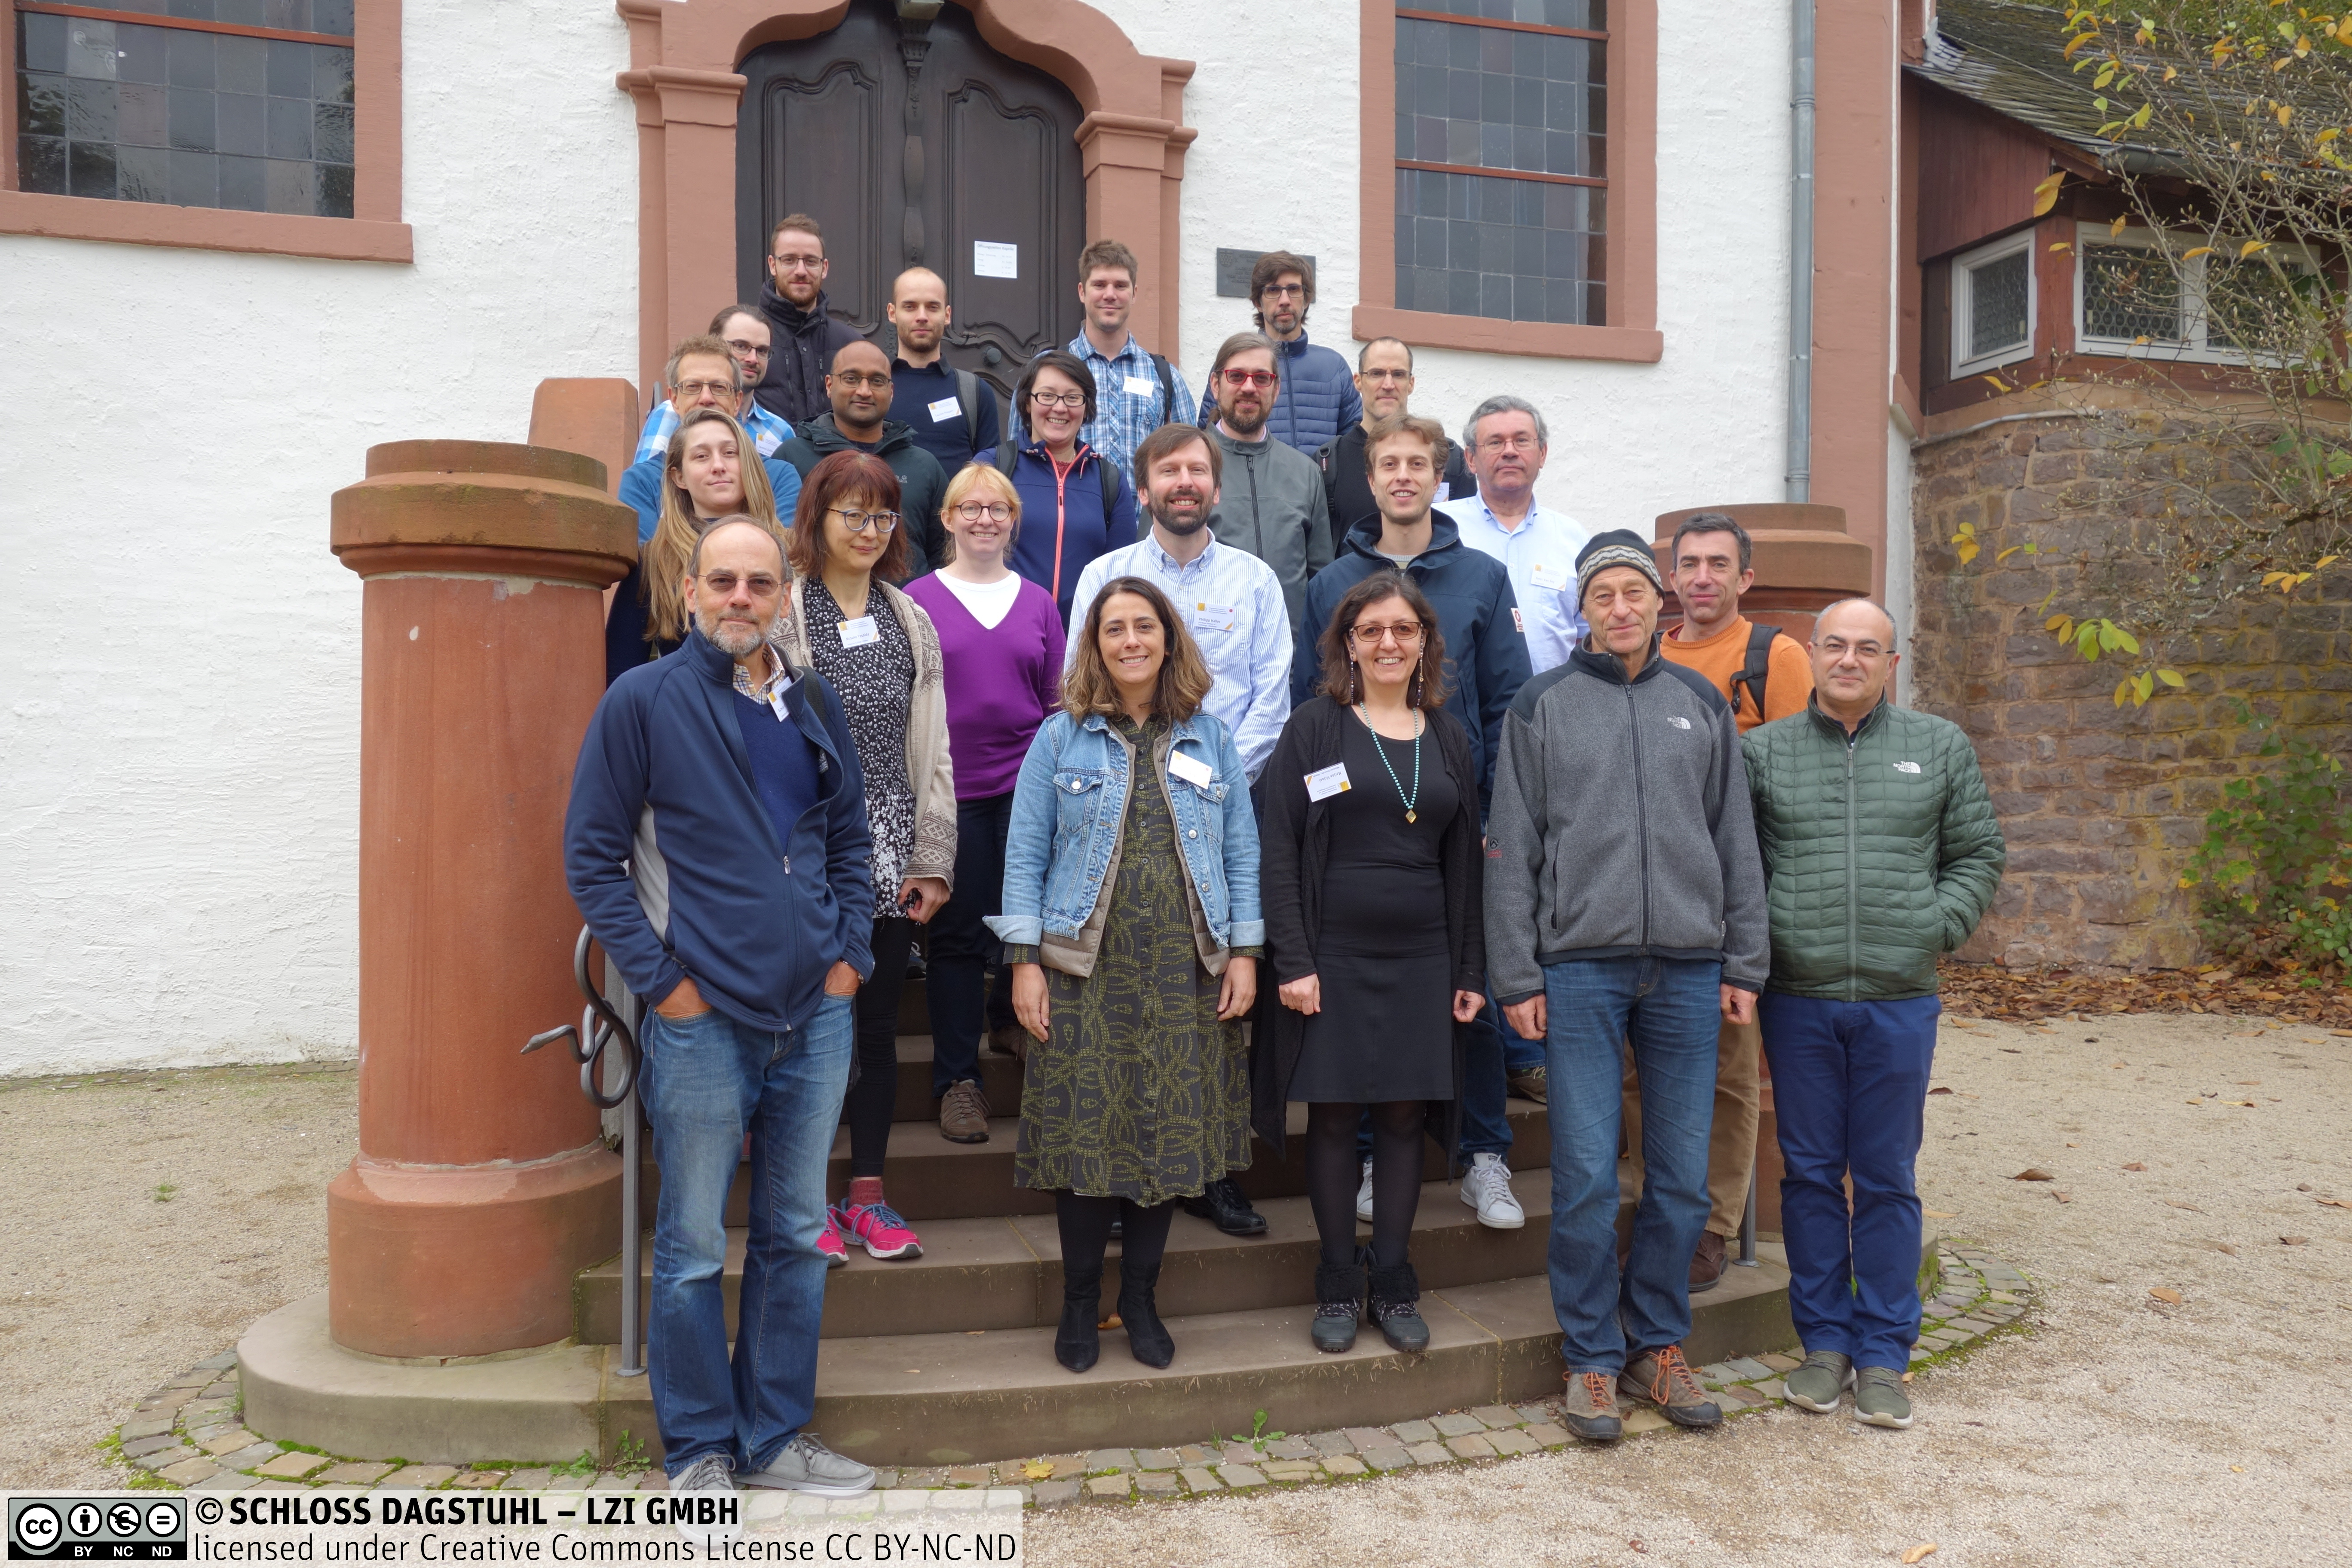
\includegraphics[width=\textwidth]{group-picture}

\end{document}
